\documentclass[]{article}
\usepackage[a4paper, total={15cm,23cm}]{geometry}
\usepackage{fancyhdr}
\usepackage{graphicx}
\usepackage{amsmath}
\usepackage{amssymb}
\usepackage{xcolor}
\usepackage{tikz}
\usepackage{verbatim}
\usepackage{tcolorbox}
\usepackage{textcomp}
\usepackage{xcomment}
\usepackage{xstring}
\usepackage{array}
%opening
\title{Vector Addition and Subtraction}
\author{Benjamin Bauml}
\date{Winter 2025}
\pagestyle{fancy}
\rhead{PH 221}
\chead{Winter 2025}
\lhead{Week 1}

% Version 2024-02-21
% Changes
% 2024-02-21 Added xstring package to enable smooth implementation of new \ModePage command.
% For Assignment, leave Purpose as 1. For Worksheet, set to 2. For Student Solution, set to 3. For Teacher Solution, set to 4.
\newcommand{\Purpose}{4}

\newcommand{\Exclusion}{0}
\newcommand{\PageTurn}{0}
\newcommand{\GrayProb}{0}
\newcommand{\Tipsy}{0}

% Assignment
\if\Purpose1
\renewcommand{\Exclusion}{1}
\fi
% Worksheet
\if\Purpose2
\renewcommand{\Exclusion}{1}
\renewcommand{\PageTurn}{1}
\fi
% Student Solution
\if\Purpose3
\renewcommand{\PageTurn}{1}
\renewcommand{\GrayProb}{1}
\fi
% Teaching Copy
\if\Purpose4
\renewcommand{\PageTurn}{1}
\renewcommand{\GrayProb}{1}
\renewcommand{\Tipsy}{1}
\fi

\if\Exclusion1
\xcomment{Title,Problem,ProblemSub,PassFig}
\fi

\def \NewQ {0}
\def \PForce {0}
\newcommand{\MaybePage}[1]{
	\def \PForce {#1}
	\if\PForce1
		\newpage
	\else
		\if\NewQ0
		\gdef \NewQ {\PageTurn}
		\else
		\newpage
		\fi
	\fi
}

\newcommand{\ModePage}[1]{
	\IfSubStr{#1}{\Purpose}{\newpage}{}
}

\newenvironment{Problem}[2][0]{%The first argument is optional, and if it is set to 1, the \newpage will be forced.
\MaybePage{#1}
\section*{#2}
\if\GrayProb1
\begin{tcolorbox}[colback=lightgray,colframe=lightgray,sharp corners,boxsep=1pt,left=0pt,right=0pt,top=0pt,bottom=0pt,after skip=2pt]
\else
\begin{tcolorbox}[colback=white,colframe=white,sharp corners,boxsep=1pt,left=0pt,right=0pt,top=0pt,bottom=0pt,after skip=2pt]
\fi
}{
\end{tcolorbox}\noindent
}

\newenvironment{ProblemSub}[1][0]{%The argument is optional, and if a string of numbers is entered into it, it will force a \newpage in any \Purpose that shows up in the string. For example, "13" would lead to the newpage being forced in modes 1 and 3.
\ModePage{#1}
\if\GrayProb1
\begin{tcolorbox}[colback=lightgray,colframe=lightgray,sharp corners,boxsep=1pt,left=0pt,right=0pt,top=0pt,bottom=0pt,after skip=2pt]
\else
\begin{tcolorbox}[colback=white,colframe=white,sharp corners,boxsep=1pt,left=0pt,right=0pt,top=0pt,bottom=0pt,after skip=2pt]
\fi
}{
\end{tcolorbox}\noindent
}

\newenvironment{PassFig}{\begin{figure}[h]}{\end{figure}}

\newcommand{\TeachingTips}[1]{
\if\Tipsy1
\begin{tcolorbox}[colback=lightgray,colframe=black]
#1
\end{tcolorbox}
\fi
}

\newenvironment{Title}{\maketitle}{}

\begin{document}
\begin{Title}
\begin{center}
	This material is borrowed/adapted from the \textit{Learning Introductory Physics with Activities} textbook.
\end{center}
\end{Title}

\begin{Problem}{Activity}
	In the following figure, the magnitudes of the vectors are $|\vec{a}| = 5$ and $|\vec{b}|=5$. Assume that $\vec{c}=\vec{a}+\vec{b}$ and $\vec{d}=\vec{a}-\vec{b}$.
\end{Problem}
\begin{PassFig}
	\centering
	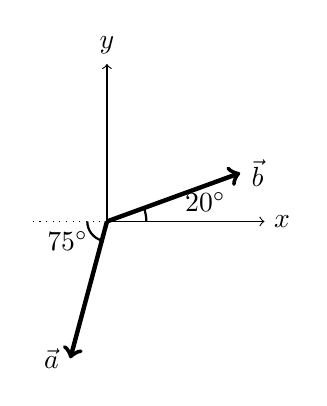
\begin{tikzpicture}
		\draw[<->] (0,2) node[anchor=south] {$y$} -- (0,0) -- (2,0) node[anchor=west] {$x$};
		\draw[->,ultra thick,rotate=20] (0,0) -- (1.8,0) node[anchor=west] {$\vec{b}$};
		\draw[->,ultra thick,rotate=255] (0,0) -- (1.8,0) node[anchor=east] {$\vec{a}$};
		\draw[dotted] (0,0) -- (-1,0);
		\draw[thick] (-0.25,0) arc (180:255:0.25);
		\node[anchor=north] at (-0.5,0) {$75^{\circ}$};
		\draw[thick] (0.5,0) arc (0:20:0.5);
		\node[anchor=south] at (1.25,0) {$20^{\circ}$};
	\end{tikzpicture}
\end{PassFig}
\begin{ProblemSub}
	Determine the magnitude of the vectors $\vec{c}$ and $\vec{d}$. What is the angle to each vector from the positive $x$-axis?
\end{ProblemSub}
To begin, let us make some visual representations of vector addition. We can estimate the quantities in question and use them to validate our final answers.
\begin{figure}[h]
	\centering
	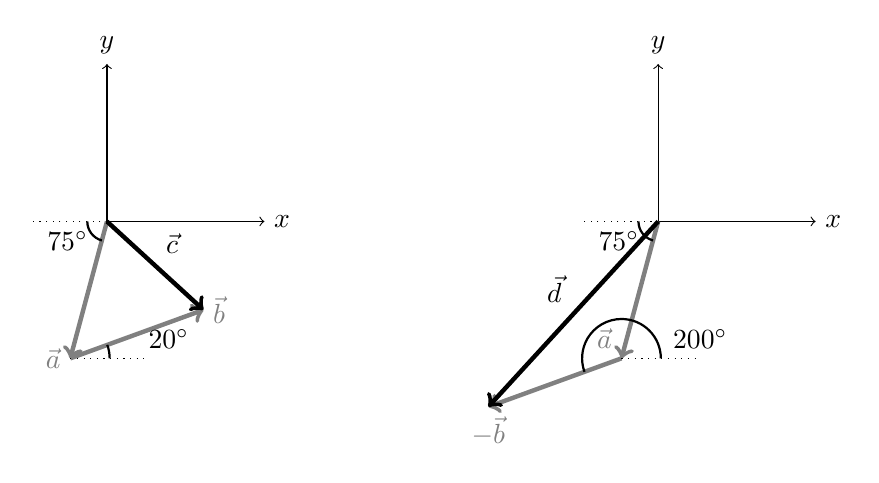
\begin{tikzpicture}
		\begin{scope}
		\draw[<->] (0,2) node[anchor=south] {$y$} -- (0,0) -- (2,0) node[anchor=west] {$x$};
		\draw[->,ultra thick,rotate=255,gray] (0,0) -- (1.8,0) node (atip) {};
		\node[anchor=east,gray] at (atip) {$\vec{a}$};
		\begin{scope}[shift={(atip)}]
		\draw[->,ultra thick,rotate=20,gray] (0,0) -- (1.8,0) node (btip) {};
		\node[anchor=west,gray] at (btip) {$\vec{b}$};
		\draw[thick] (0.5,0) arc (0:20:0.5);
		\node[anchor=south] at (1.25,0) {$20^{\circ}$};
		\draw[dotted] (0,0) -- (1,0);
		\end{scope}
		\draw[dotted] (0,0) -- (-1,0);
		\draw[thick] (-0.25,0) arc (180:255:0.25);
		\node[anchor=north] at (-0.5,0) {$75^{\circ}$};
		\draw[->,ultra thick,rotate=-42.5] (0,0) -- (0.82,0) node[anchor=south west] {$\vec{c}$} -- (1.66,0);
		\end{scope}
		\begin{scope}[shift={(7,0)}]
			\draw[<->] (0,2) node[anchor=south] {$y$} -- (0,0) -- (2,0) node[anchor=west] {$x$};
			\draw[->,ultra thick,rotate=255,gray] (0,0) -- (1.8,0) node (atip) {};
			\node[anchor=south east,gray] at (atip) {$\vec{a}$};
			\begin{scope}[shift={(atip)}]
				\draw[->,ultra thick,rotate=200,gray] (0,0) -- (1.8,0) node (btip) {};
				\node[anchor=north,gray] at (btip) {$-\vec{b}$};
				\draw[thick] (0.5,0) arc (0:200:0.5);
				\node[anchor=south] at (1,0) {$200^{\circ}$};\draw[dotted] (0,0) -- (1,0);
			\end{scope}
			\draw[dotted] (0,0) -- (-1,0);
			\draw[thick] (-0.25,0) arc (180:255:0.25);
			\node[anchor=north] at (-0.5,0) {$75^{\circ}$};
			\draw[->,ultra thick,rotate=227.5] (0,0) -- (1.6,0) node[anchor=south east] {$\vec{d}$} -- (3.19,0);
		\end{scope}
	\end{tikzpicture}
\end{figure}

We can see that $\vec{c}$ will be slightly smaller than 5 units long, and nearly 45$^{\circ}$ below the positive $x$-axis, while $\vec{d}$ will be probably close to 9 units long (almost twice 5, based on my visual estimate) and around 135$^{\circ}$ below the positive $x$-axis.

To begin, let us break down the known vectors into their components. Note that the angle $\vec{a}$ makes is with respect to the negative $x$-axis and below it, so an explicit negative sign will be added both components.
\[
\begin{split}
	a_{x} & = -5\cos(75^{\circ}) \approx -1.29, \\
	a_{y} & = -5\sin(75^{\circ}) \approx -4.83, \\
	b_{x} & = 5\cos(20^{\circ}) \approx 4.70, \\
	b_{y} & = 5\sin(20^{\circ}) \approx 1.71.
\end{split}
\]
Adding the vectors componentwise, we obtain
\[
\begin{split}
	\vec{c} & = \vec{a}+\vec{b} \approx 3.41 \hat{x} - 3.12 \hat{y}, \\
	\vec{d} & = \vec{a}-\vec{b} \approx -5.99 \hat{x} - 6.54 \hat{y}.
\end{split}
\]
We can then use the Pythagorean theorem to calculate the magnitudes of these vectors:
\[
\begin{split}
	|\vec{c}| & \approx \sqrt{3.41^{2}+3.12^{2}} \approx 4.62, \\
	|\vec{d}| & \approx \sqrt{5.99^{2}+6.54^{2}} \approx 8.87.
\end{split}
\]
Trigonometry can be used to find the directions of these vectors. For $\vec{c}$, let the angle from the positive $x$-axis be
\[
\gamma \approx \arctan\left(\frac{-3.12}{3.14}\right) \approx -42.5^{\circ},
\]
therefore $\vec{c}$ points 42.5$^{\circ}$ below the positive $x$-axis. For $\vec{d}$, let the angle from the positive $x$-axis be
\[
\delta^{*} = \approx \arctan\left(\frac{-6.54}{-5.99}\right) \approx 47.5^{\circ}.
\]
However, this points into the first quadrant, which we know is incorrect. The tangent function is tricky that way. It has a period of 180$^{\circ}$, so there is more than one angle that gives the same result, and the inverse tangent is not guaranteed to give you the right one. We can subtract the period to get another valid answer:
\[
\delta = \delta^{*} - 180^{\circ} \approx -132.5^{\circ},
\]
therefore $\vec{d}$ points 132.5$^{\circ}$ below the positive $x$-axis.
\end{document}